\section{Working with GIT}

\subsection{Overview of GIT-commands}

The following picture will give a good overview over the workflow and the commands in GIT:\\
\begin{figure}[h!]
 \begin{center}
  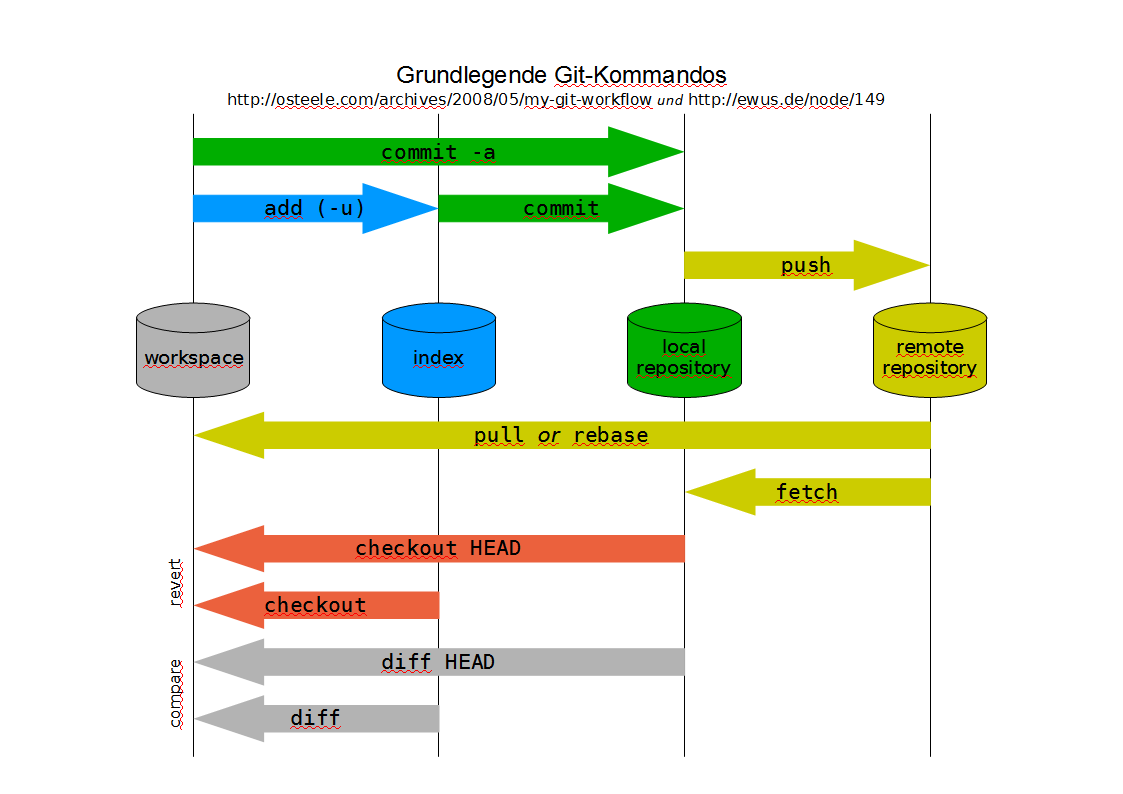
\includegraphics[width=12cm,height=9cm]{./pics/git.png}
 \end{center}
 \caption{An Overview over GIT commands}
\end{figure}
The main advantage in GIT is, that every host has got his own local repository, which in itself is an external repository to another host.\newpage 
I will give an example, in which I will try, to use most of the commands GIT gives us:
\begin{itemize}
 \item You create a new file in your workspace in your own branch, that was not under version control before
 \item Now you first have to add it to the \emph{index}, which for GIT is just a list of files, that it has to monitor. You can do this using \emph{add}
 \item The next step is adding the actual file to the local repository. You can do this via \emph{commit}
 \item Now the file is under version control. You can now could get the file from the repository using \emph{checkout HEAD}
 \item If you also want to add the file to the remote repository, you can use \emph{push}
 \item Now another person can get your whole work using \emph{pull}, which will provide him with everything, that is currently listed in your \emph{remote repository}
\end{itemize}
\remph{Please note: Be careful whilst merging, Eclipse will offer you to ``overwrite'', which is not a good idea, as it does exactly what it promisses instead of merging. We will support this warning with a screenshot if possible!}
To provide a full overview over the commands, I will list all the commands, that Eduard did show us in his presentation:
\begin{itemize}
 \item \emph{git add}: adds file changes in your workspace to your index
 \item \emph{git commit}: Commits all the changes listed in the index to the local repository
 \item \emph{git push}: Pushes local branch to the remote repository
 \item \emph{git fetch}: Fetches all files from the remote repository, that are not in the local repository
 \item \emph{git merge}: Merges one or more branches into your current branch
 \item \emph{git pull}: Fetches files from remote repository and merges them with local files (equal to \emph{git fetch; git merge})
 \item \emph{git rm}: Removes a file from your repository 
\end{itemize}
\newpage
\subsection{Setting up your own branch with GIT}
Within your repository, you should still create branches for each feature you develop.
To create a new branch you simple do:
\begin{enumerate}
 \item In Eclipse, right-click on \emph{name\_of\_your\_fork}
 \item Select \emph{Team}$\rightarrow$\emph{Switch to}$\rightarrow$\emph{New Branch} 
 \item As shown in the picture bellow, select the source:\\ \emph{refs/remotes/origin/goettingen\_master}\footnote{By choosing this, you make sure, that you have the latest online version} 
% Hier nachfragen, wie das ganze jetzt ist, mit MASTER und GOETTINGEN_MASTER  
 \item Choose a name following the scheme yourname\_yourfeature
 \item Activate the checkbox for checking out the new branch
 \item Work away
\end{enumerate}

\begin{figure}[h!]
 \begin{center}
 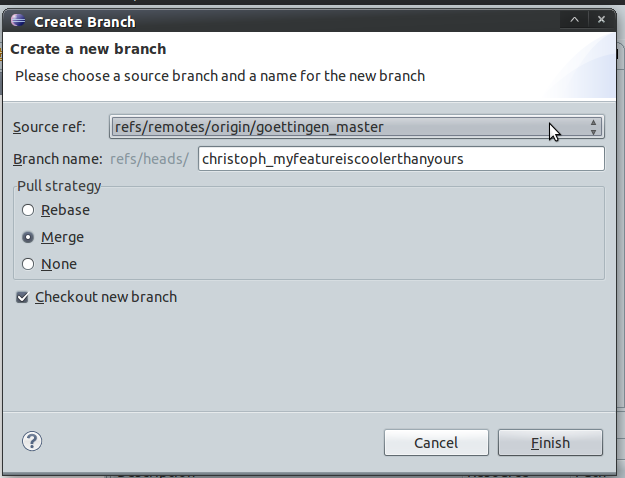
\includegraphics[height=8cm]{./pics/NewBranchSmall.png}
\end{center}
\caption{How to create a new branch within Eclipse}
\end{figure}



\newpage

\subsection{Forking a Repository}
\label{forksection}
To create a fork of a repository, you need access to the assembla-website. Once you have logged in, you can choose a repository and then click on the button \emph{fork network}.
One click on the button \emph{fork} will then create a fork of the repository for you, as shown in Figure \ref{fork}. You will furthermore be asked for a name of this copy of the repository, remember this name, as you will need it for the setup!

\begin{figure}[h!]
\begin{center}
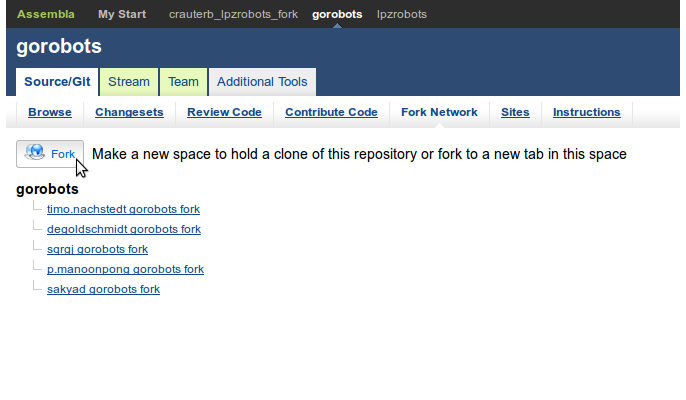
\includegraphics[width=12cm]{./pics/Fork.png}
\caption{How to fork a repository at the Assembla website}
\label{fork}
\end{center}
\end{figure}

\subsection{Merging}
Please check with your supervisor, before merging back into \emph{master}. \\
If you want to merge a branch of yours, you will have to send a merge request via the assembla-webpage. A supervisor will then have a look at your code. \emph{BUT} he is only able to do so,
if you have given him or her the rights to read your code. You can do so by, on the assembla-webpage in your forked repository, select \emph{team} and then, on the right, select \emph{Invite people from other teams}.
No you can choose which one you want to invite, and then you can choose which rights you want to give him or her.

\subsection{How to update your Master Branch}

Make sure that you are in your master branch by typing:
\begin{lstlisting}
~/workspace/YOURLOGIN-gorobots-fork $ git branch
\end{lstlisting}
The output should be something like this:
\begin{lstlisting}
  goplus
  feature_branch_1
  feature_branch_2
  feature_branch_3
* master 
\end{lstlisting}
The star indicates, in which branch you are working right now. If you are not working in the \emph{master}-branch, switch to the branch by typing:
\begin{lstlisting}
 ~/workspace/YOURLOGIN-gorobots-fork $ git checkout master
\end{lstlisting}
You can use \emph{git branch} again, to check of you are in the right branch now.

If you are in the master branch type
\begin{lstlisting}
~/workspace/YOURLOGIN-gorobots-fork$ git remote -v
\end{lstlisting}
The output should be something like this (if you did not add a remote before):
\begin{lstlisting}
origin https://YOURLOGIN@git.assembla.com/YOURLOGIN-gorobots-fork.git (fetch)
origin https://YOURLOGIN@git.assembla.com/YOURLOGIN-gorobots-fork.git (push)
\end{lstlisting}
Now you have to add a stable repository as additional remote type:
\begin{lstlisting}
git remote add stable https://YOURLOGIN@git.assembla.com/gorobots.git 
\end{lstlisting}
\emph{git remote -v} should now show something like:
\begin{lstlisting}
~/workspace/YOURLOGIN-gorobots-fork $ git remote -v
origin https://YOURLOGIN@git.assembla.com/YOURLOGIN-gorobots-fork.git (fetch)
origin https://YOURLOGIN@git.assembla.com/YOURLOGIN-gorobots-fork.git (push)
stable https://YOURLOGIN@git.assembla.com/gorobots.git (fetch)
stable https://YOURLOGIN@git.assembla.com/gorobots.git (push) 
\end{lstlisting}
This means you are able to connect to the stable repository (referred to as stable) from your local repository. \\
Now update your local repositories information about the stable repository by typing:
\begin{lstlisting}
~/workspace/YOURLOGIN-gorobots-fork $ git fetch stable  
\end{lstlisting}
After typing your password you see an output like the following:
\begin{lstlisting}
From https://git.assembla.com/gorobots
 * [new branch]      master     -> stable/master 
\end{lstlisting}
Your local repository knows now what branches are available in the stable repository.\\
Now merge the changes of the stable master in your workspace (which currently contains your local master branch) by typing:
\begin{lstlisting}
~/workspace/YOURLOGIN-gorobots-fork $ git merge stable/master 
\end{lstlisting}
If there were now changes, the Output would be something like:
\begin{lstlisting}
Already up-to-date. 
\end{lstlisting}
An example of an output including changes would look like:
\begin{lstlisting}
Updating 1054d9a..330d652
Fast-forward
 docs/README                |    6 ++++++
 docs/install_manual/README |    5 +++++
 docs/install_script/README |    6 ++++++
 3 files changed, 17 insertions(+), 0 deletions(-)
 create mode 100644 docs/README
 create mode 100644 docs/install_manual/README
 create mode 100644 docs/install_script/README 
\end{lstlisting}
Now you can use \emph{git commit}, to commit changes to your local repository, and \emph{git push}, to commit changes to the remote repository. \\
Now your master branch is up to date with our stable version and you can continue with the next section.

